\documentclass{article}
\usepackage{tikz}
\usetikzlibrary{matrix}

\begin{document}

\begin{figure}[h]
    \centering
    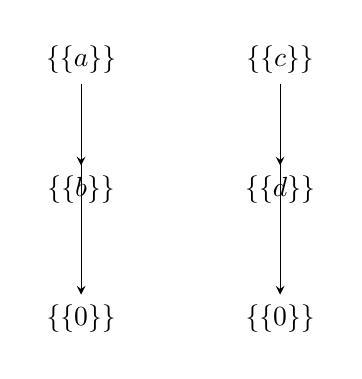
\begin{tikzpicture}
        \matrix (m) [matrix of math nodes,row sep=3em,column sep=4em,minimum width=2em] {
            \{\{a\}\} & \{\{c\}\} \\
            \{\{b\}\} & \{\{d\}\} \\
            \{\{0\}\} & \{\{0\}\} \\
        };
        \path[-stealth]
        (m-1-1) edge node [left] {} (m-2-1)
        (m-1-1) edge node [left] {} (m-3-1)
        (m-1-2) edge node [left] {} (m-2-2)
        (m-1-2) edge node [left] {} (m-3-2);
    \end{tikzpicture}
    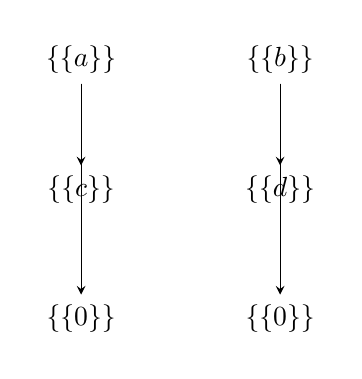
\begin{tikzpicture}
        \matrix (m) [matrix of math nodes,row sep=3em,column sep=4em,minimum width=2em] {
            \{\{a\}\} & \{\{b\}\} \\
            \{\{c\}\} & \{\{d\}\} \\
            \{\{0\}\} & \{\{0\}\} \\
        };
        \path[-stealth]
        (m-1-1) edge node [left] {} (m-2-1)
        (m-1-1) edge node [left] {} (m-3-1)
        (m-1-2) edge node [left] {} (m-2-2)
        (m-1-2) edge node [left] {} (m-3-2);
    \end{tikzpicture}
    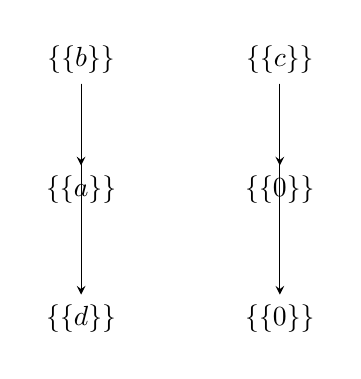
\begin{tikzpicture}
        \matrix (m) [matrix of math nodes,row sep=3em,column sep=4em,minimum width=2em] {
            \{\{b\}\} & \{\{c\}\} \\
            \{\{a\}\} & \{\{0\}\} \\
            \{\{d\}\} & \{\{0\}\} \\
        };
        \path[-stealth]
        (m-1-1) edge node [left] {} (m-2-1)
        (m-1-1) edge node [left] {} (m-3-1)
        (m-1-2) edge node [left] {} (m-2-2)
        (m-1-2) edge node [left] {} (m-3-2);
    \end{tikzpicture}
    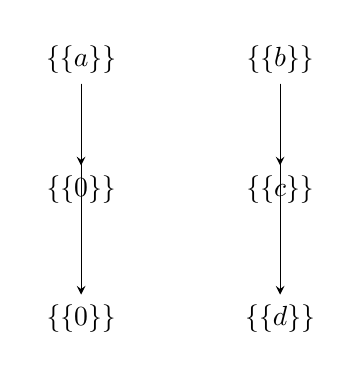
\begin{tikzpicture}
        \matrix (m) [matrix of math nodes,row sep=3em,column sep=4em,minimum width=2em] {
            \{\{a\}\} & \{\{b\}\} \\
            \{\{0\}\} & \{\{c\}\} \\
            \{\{0\}\} & \{\{d\}\} \\
        };
        \path[-stealth]
        (m-1-1) edge node [left] {} (m-2-1)
        (m-1-1) edge node [left] {} (m-3-1)
        (m-1-2) edge node [left] {} (m-2-2)
        (m-1-2) edge node [left] {} (m-3-2);
    \end{tikzpicture}
    \caption{For the semigroup $U_2$, the posets of $\mbox{${\mathcal{L}}$}$-classes (left), $\mbox{${\mathcal{R}}$}$-classes (middle left), $\mbox{${\mathcal{J}}$}$-classes (middle right) and $\mbox{${\mathcal{H}}$}$-classes (right).}
    \label{fig:posets}
\end{figure}

\end{document}